\begin{titlepage}

\chapter{Introducción}
\section{Introducción y motivación}
A día de hoy, el coste de la electricidad ha aumentado a unos niveles que nadie hubiera imaginado hace tan solo unos años. Muchas familias cada vez más, necesitan ir con mucho cuidado sobre cuándo poner ciertos electrodomésticos en casa, para elegir la hora donde el precio está más bajo y así poder ahorrar en la factura de la luz. Saber cuánto consume cada electrodoméstico y como se refleja en el coste de la factura puede llegar a ser de gran utilidad. \\

Y aquí es donde podemos situar el trabajo de este proyecto. Aunque a día de hoy existen sistemas inteligentes con los que gestionar y monitorizar la energía que se consume en el hogar, normalmente estos dispositivos son independientes unos de otros y no encontramos muchos que recopilen los datos. Estos dispositivos que ya existen en el mercado los analizaremos más adelante. El trabajo de este proyecto, no solo se va a centrar en medir el consumo eléctrico de los dispositivos individualmente, si no que el objetivo será que toda esa información se pueda consultar desde una misma aplicación. \\

En este proyecto se plantea el despliegue de diferentes sistemas embebidos, que se comunicaran con un servidor que recopile toda la información.\\

\section{Objetivos}

\begin{enumerate}
\item Estudio de viabilidad de la plataforma de desarrollo. Uso de micropython y estudio de la existencia de librerias para la comunicación inalámbrica por MQTT.
\item Estudio de los diferentes dispositivos que se pueden utilizar para medir el consumo eléctrico. 
\item Puesta a punto de raspberry pi para el despliegue de un broker MQTT.
\item Integración de los sensores y dispositivos con la plataforma elegida.
\item Aplicación web en FLask que permita la visualización de los datos recogidos por los dispositivos en tiempo real.
\end{enumerate}

\section{Planificación}
La planificación inicial y el tiempo estimado a emplear en cada tarea fue el siguiente:
\begin{figure}[h!]
	\centering
	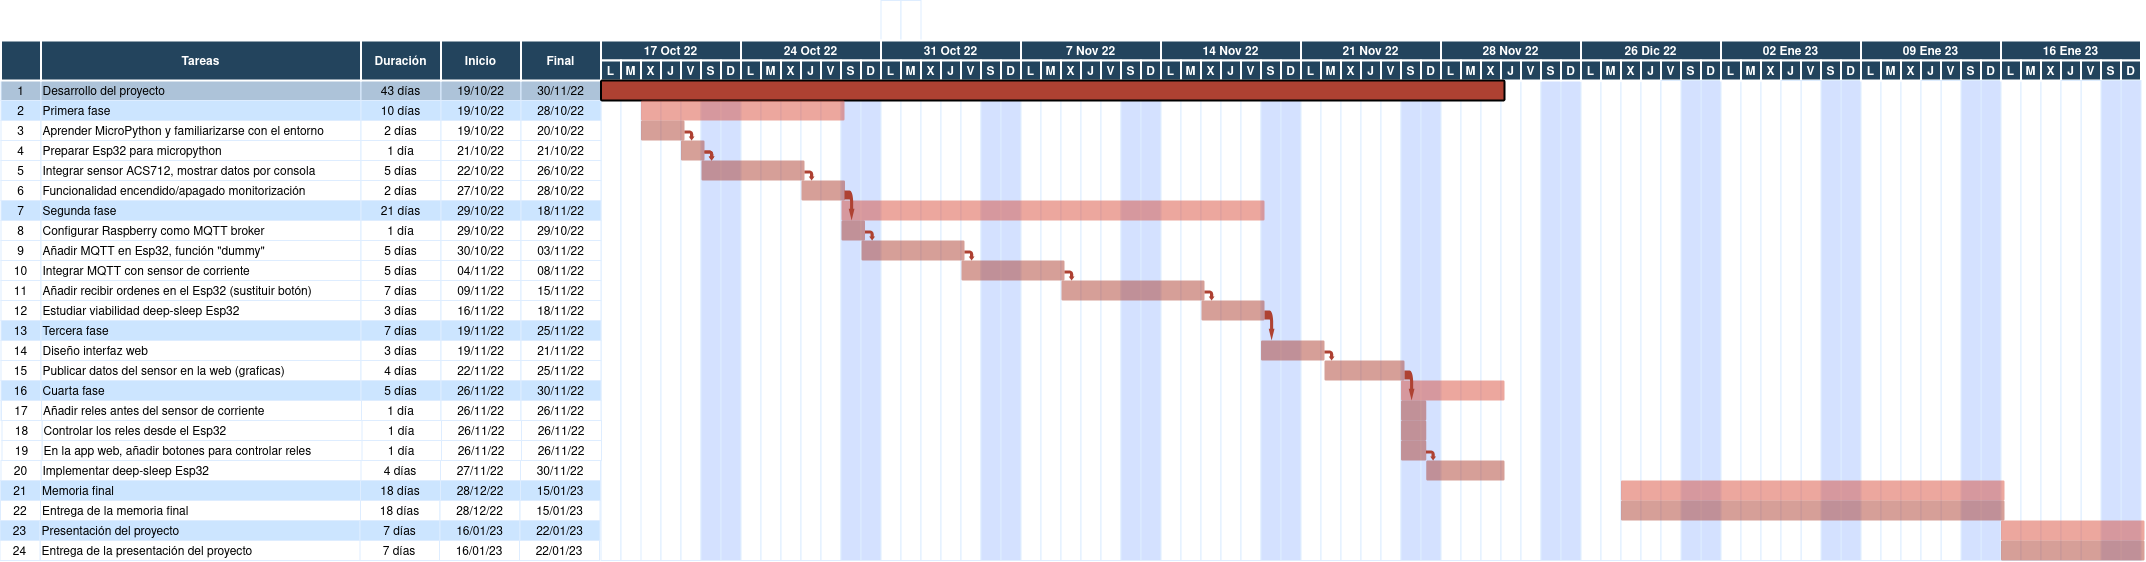
\includegraphics[width=1\textwidth]{imagenes/gantt_inicial.PNG}
	\caption{Diagrama de Gantt para la planificación inicial}
\end{figure}
Hasta el momento, se han cumplido la mayoria de objetivos planificados, aunque se han tenido que retrasar algunas tareas debido a la falta de tiempo. A continuación se muestra la planificación actualizada:
Insertar imagen con nueva planificación

\section{Material y métodos}
\subsubsection{Software}
\begin{itemize}
	\item Visual Studio Code como IDE de programación.
	\item Ordenador con Ubuntu como SO.
	\item Esptool como herramienta para trabajar con la flash de los ESP32.
	\item Para la creación de este documento se ha utilizado Texmaker como plataforma de creación y edición de documentos \LaTeX
	\item Picocom como software para la comunicación por serial.
\end{itemize}

\subsubsection{Equipos}
\begin{itemize}
	\item Raspberry Pi 2B+ como broker MQTT.
	\item x3 ESP32.
	\item x3 sensores de corriente ACS712.
	\item x3 sensores de voltaje. 
	\item x3 pantallas OLED SSD1306.
	\item x3 cables USB - Micro USB.
	\item X3 reles.
	\item Multimetro
	\item Fuente de alimentación.
	\item x6 Mini breadboards.
	\item Otros componentes electronicos.
\end{itemize}

\section{Estructura del documento}
El documento se divide en 5 capítulos, que se describen a continuación:
\begin{enumerate}
\item Capítulo 1. Introducción. En este capítulo se describen los objetivos del proyecto, así como la planificación inicial y la planificación actualizada. También se describen los materiales y métodos utilizados para la realización del proyecto. 
\item Capítulo 2. Estudio del problema. En este capítulo se describen los diferentes dispositivos que se pueden utilizar para medir el consumo eléctrico. También se describen los diferentes protocolos de comunicación que se pueden utilizar para la comunicación entre los dispositivos y el servidor.
\item Capítulo 3. Implementación del sistema de monitorización de corriente. En este capítulo se describe la solución final, los materiales utilizados, el setup experimental y la implementación en Micropython.
\item Capítulo 4. Implementación de la aplicación web. En este capítulo se describe la implementación de la aplicación web en Python usando Flask, SocketIO y MQTT.
\item Capítulo 5. Conclusiones y trabajo futuro. En este capítulo se describen las conclusiones del proyecto y las posibles mejoras que se podrían realizar en el futuro.
\end{enumerate}

\end{titlepage}
